\documentclass[tikz, border=10pt]{standalone}
\usetikzlibrary{arrows, positioning, calc}

\begin{document}

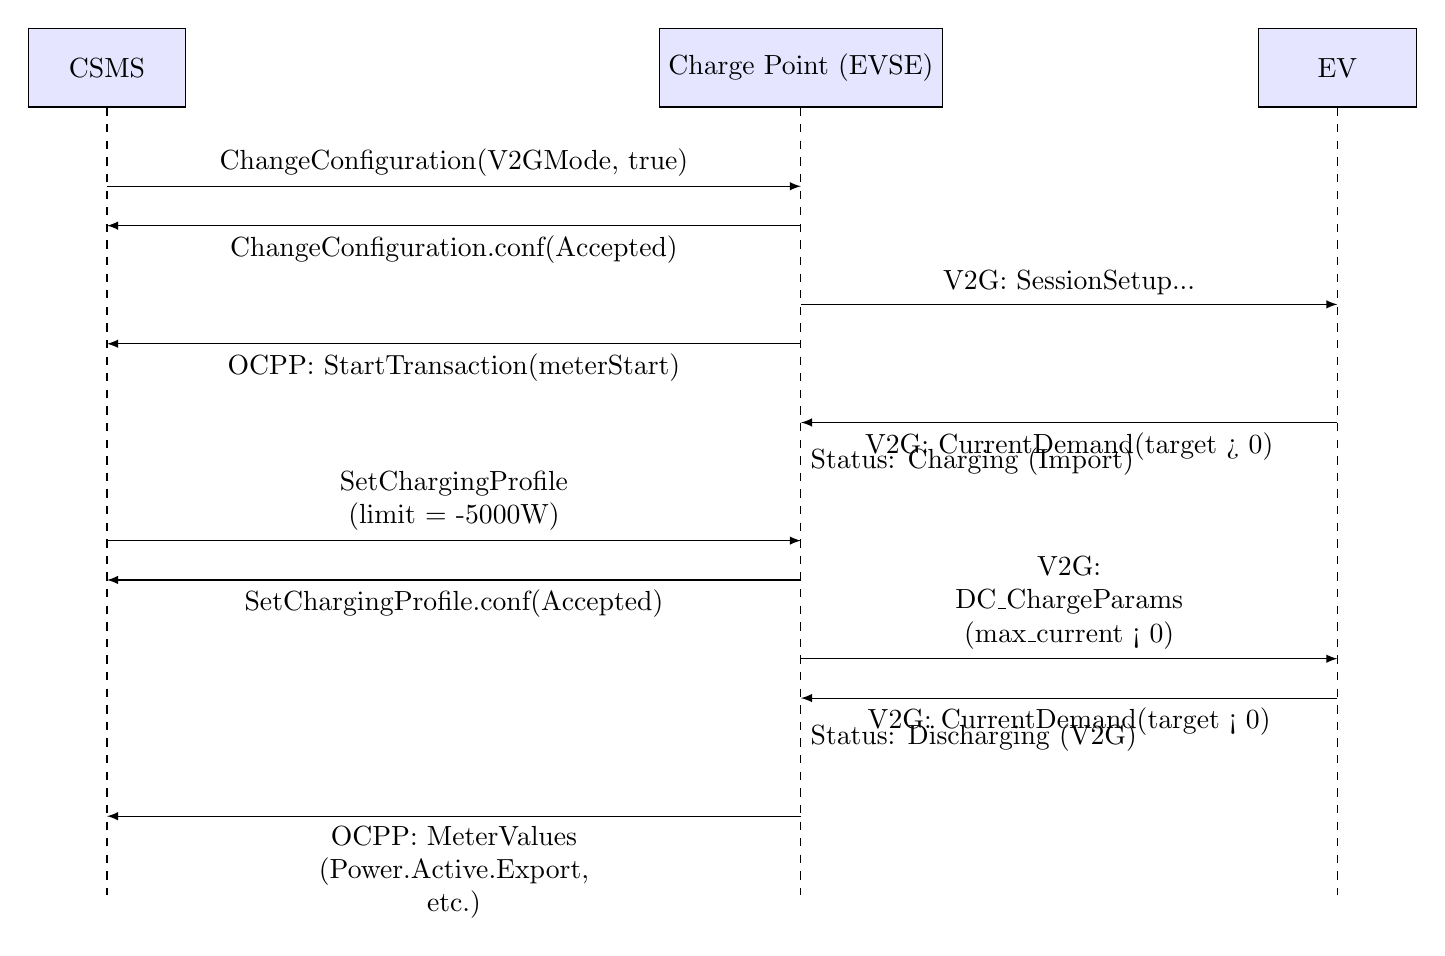
\begin{tikzpicture}[>=stealth', auto]
  % Styles
  \tikzstyle{actor} = [rectangle, draw, minimum width=2cm, minimum height=1cm, fill=blue!10]
  \tikzstyle{line} = [draw, -]
  \tikzstyle{message} = [draw, ->, >=latex]
  
  % Actors
  \node[actor] (CSMS) {CSMS};
  \node[actor, right=6cm of CSMS] (CP) {Charge Point (EVSE)};
  \node[actor, right=4cm of CP] (EV) {EV};

  % Lifelines
  \draw[line, dashed] (CSMS.south) -- +(0,-10);
  \draw[line, dashed] (CP.south) -- +(0,-10);
  \draw[line, dashed] (EV.south) -- +(0,-10);

  % --- Sequence Start ---

  % 1. V2G Mode Enable
  \draw[message] ($(CSMS.south)+(0,-1)$) -- node {ChangeConfiguration(V2GMode, true)} ($(CP.south)+(0,-1)$);
  \draw[message] ($(CP.south)+(0,-1.5)$) -- node {ChangeConfiguration.conf(Accepted)} ($(CSMS.south)+(0,-1.5)$);

  % 2. Start Charging (Normal)
  \draw[message] ($(CP.south)+(0,-2.5)$) -- node {V2G: SessionSetup...} ($(EV.south)+(0,-2.5)$);
  \draw[message] ($(CP.south)+(0,-3.0)$) -- node {OCPP: StartTransaction(meterStart)} ($(CSMS.south)+(0,-3.0)$);

  % 3. Charging (Import)
  \draw[message] ($(EV.south)+(0,-4.0)$) -- node {V2G: CurrentDemand(target > 0)} ($(CP.south)+(0,-4.0)$);
  \node at ($(CP.south)+(0,-4.5)$) [right] {Status: Charging (Import)};

  % 4. V2G Export Trigger (Signed Limit)
  \draw[message] ($(CSMS.south)+(0,-5.5)$) -- node [text width=3.5cm, align=center] {SetChargingProfile\\(limit = -5000W)} ($(CP.south)+(0,-5.5)$);
  \draw[message] ($(CP.south)+(0,-6.0)$) -- node {SetChargingProfile.conf(Accepted)} ($(CSMS.south)+(0,-6.0)$);

  % 5. V2G Export Behavior
  \draw[message] ($(CP.south)+(0,-7.0)$) -- node [text width=3cm, align=center] {V2G: DC\_ChargeParams\\(max\_current < 0)} ($(EV.south)+(0,-7.0)$);
  \draw[message] ($(EV.south)+(0,-7.5)$) -- node {V2G: CurrentDemand(target < 0)} ($(CP.south)+(0,-7.5)$);
  \node at ($(CP.south)+(0,-8.0)$) [right] {Status: Discharging (V2G)};

  % 6. Metering
  \draw[message] ($(CP.south)+(0,-9.0)$) -- node [text width=3.5cm, align=center] {OCPP: MeterValues\\(Power.Active.Export, etc.)} ($(CSMS.south)+(0,-9.0)$);

\end{tikzpicture}

\end{document}
